\documentclass[11pt,a4paper]{article}

% --- Packages ---
\usepackage[margin=2.5cm]{geometry}
\usepackage{amsmath,amssymb}
\usepackage{booktabs}
\usepackage{graphicx}
\usepackage{listings}
\usepackage{xcolor}
\usepackage{hyperref}
\usepackage[backend=biber,style=numeric,sorting=none,date=long,urldate=long]{biblatex}
\addbibresource{refs.bib}
\usepackage{caption}
\usepackage{float}
\usepackage{tikz}
\usepackage{longtable}
\usepackage{array}

% Code listing style for C++ / GLSL / OpenGL
\lstset{
  basicstyle=\ttfamily\small,
  keywordstyle=\color{blue}\bfseries,
  commentstyle=\color{gray},
  stringstyle=\color{red!70!black},
  numbers=left,
  numberstyle=\tiny\color{gray},
  numbersep=5pt,
  frame=single,
  breaklines=true,
  tabsize=4,
  showstringspaces=false,
  language=C++
}

\title{IN3005 Interim Coursework\\[0.3em]
       \large Solar Sail Panel}
\author{Anker Rasmussen \\ 230022888}
\date{\today}

\begin{document}
\maketitle

\begin{figure}[H]
  \centering
  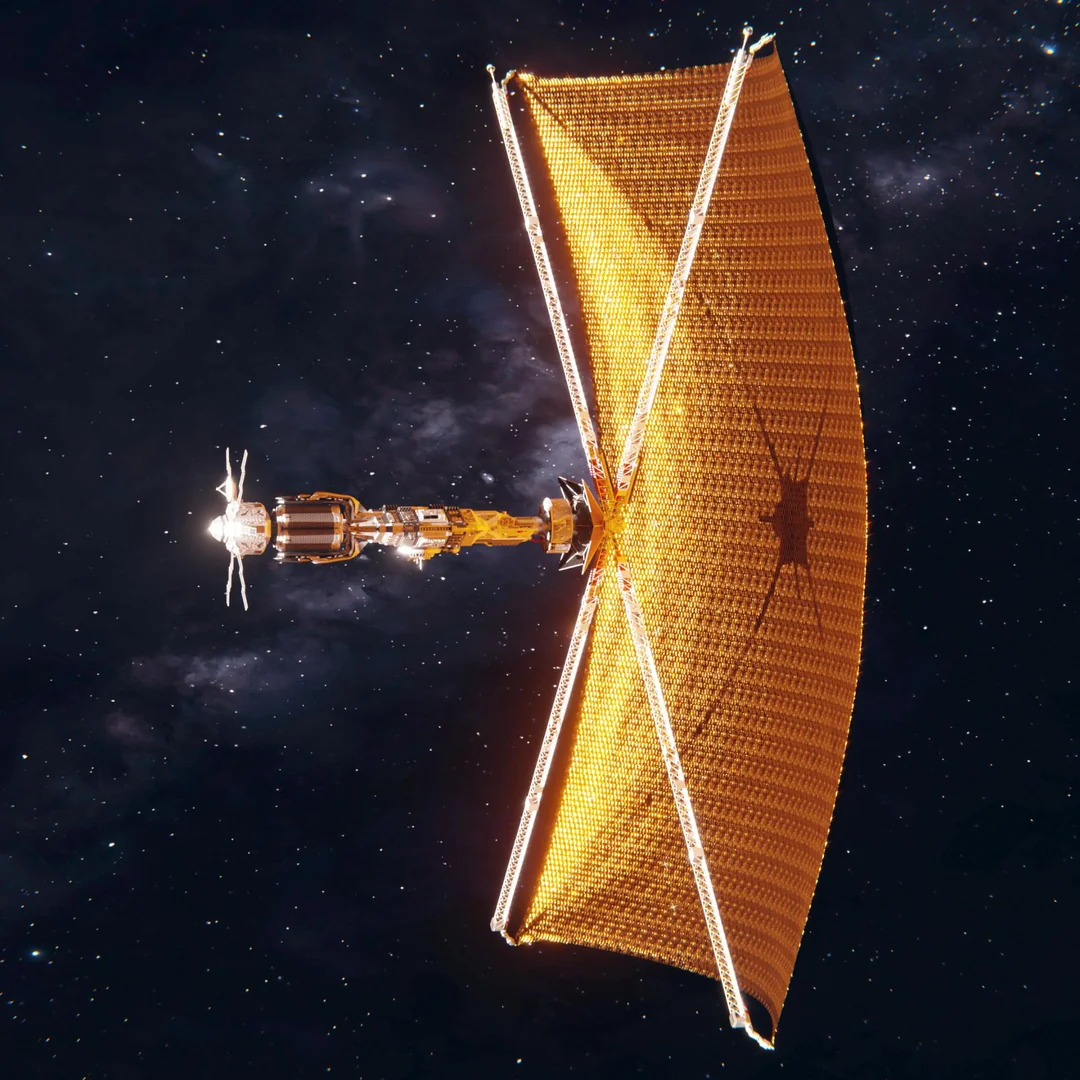
\includegraphics[width=0.6\textwidth]{img/Ship.png}
  \caption{Blender render by u/mstx~\cite{reddit_solarsail} that inspired the solar sail design.}
  \label{fig:inspiration}
\end{figure}

\noindent
The choice of a solar sail was inspired by this render,
which modelled a spacecraft with a large solar sail.
For this interim coursework only one of my proposed sail panels are modelled.
As depicted in the spaceship image, the body would sit behind it, dictating the sail's orientation and motion.
The choice to make the sail curved was personal. 
Note: a curved surface does not
capture more sunlight than a flat square of the same span (less surface area),
but it makes for a more interesting shape to model and looks cooler (physics is an afterthought).


% ======================================================================
\section{Task 1: Object Definition}
% ======================================================================

The object I picked is one of the \textbf{solar sail panels} for a spaceship,
defined as a Coons patch~\cite{farin2002coons,ye2003coons} with cubic B\'{e}zier boundary curves~\cite{farin2002bezier,pomax},
rendered double-sided (50 vertices, 64 triangles, 192 indices).
The origin is placed at the sail's aft corner so that all coordinates
are positive along the forward axis, simplifying the boundary curve setup.

\begin{figure}[H]
  \centering
  \includegraphics[width=0.85\textwidth]{img/formulae.png}
  \caption{Sail geometry sketch and associated equations.}
  \label{fig:formulae}
\end{figure}

% ----------------------------------------------------------------------
\subsection{Corners and Boundary Curves}
% ----------------------------------------------------------------------

\begin{center}
\begin{tabular}{lccc}
\toprule
Corner & Index & $(s,\,t)$ & Position \\
\midrule
Aft  & V0  & $(0,0)$ & $(0,\;2,\;5)$ \\
LatB & V4  & $(1,0)$ & $(4,\;1,\;9)$ \\
LatA & V20 & $(0,1)$ & $(-4,\;1,\;9)$ \\
Fwd  & V24 & $(1,1)$ & $(0,\;0,\;13)$ \\
\bottomrule
\end{tabular}
\end{center}

Each edge is a cubic B\'{e}zier curve
$\mathbf{B}(u) = (1\!-\!u)^3 \mathbf{P}_0 + 3(1\!-\!u)^2 u\,\mathbf{P}_1
+ 3(1\!-\!u)u^2\,\mathbf{P}_2 + u^3\,\mathbf{P}_3$.
Inner control points are at $\frac{1}{3}$/$\frac{2}{3}$ interpolation
plus bow vector $\mathbf{b} = (0,\;1.5,\;0)$:

\begin{center}
\small
\begin{tabular}{llcccc}
\toprule
Edge & Path & $\mathbf{P}_0$ & $\mathbf{P}_1$ & $\mathbf{P}_2$ & $\mathbf{P}_3$ \\
\midrule
$E_0$ & aft $\to$ latB
  & $(0, 2, 5)$ & $(1.333, 3.167, 6.333)$ & $(2.667, 2.833, 7.667)$ & $(4, 1, 9)$ \\
$E_1$ & latB $\to$ fwd
  & $(4, 1, 9)$ & $(2.667, 2.167, 10.333)$ & $(1.333, 1.833, 11.667)$ & $(0, 0, 13)$ \\
$E_2$ & fwd $\to$ latA
  & $(0, 0, 13)$ & $(-1.333, 1.833, 11.667)$ & $(-2.667, 2.167, 10.333)$ & $(-4, 1, 9)$ \\
$E_3$ & latA $\to$ aft
  & $(-4, 1, 9)$ & $(-2.667, 2.833, 7.667)$ & $(-1.333, 3.167, 6.333)$ & $(0, 2, 5)$ \\
\bottomrule
\end{tabular}
\end{center}

% ----------------------------------------------------------------------
\subsection{Coons Patch Surface}
% ----------------------------------------------------------------------

\begin{equation}\label{eq:coons}
  \mathbf{P}(s,t) = (1\!-\!t)\,\mathbf{B}_{E_0}(s) + t\,\mathbf{B}_{E_2}(1\!-\!s)
                   + (1\!-\!s)\,\mathbf{B}_{E_3}(1\!-\!t) + s\,\mathbf{B}_{E_1}(t)
                   - \mathbf{L}(s,t)
\end{equation}

where $\mathbf{L}(s,t) = (1\!-\!s)(1\!-\!t)\,C_{00} + s(1\!-\!t)\,C_{10}
+ (1\!-\!s)t\,C_{01} + st\,C_{11}$ is the bilinear corner correction.
A concavity dip $z \leftarrow z - 0.3\sin(\pi s)\sin(\pi t)$ simulates
sail billowing (zero at edges, $-0.3$ at centre).

% ----------------------------------------------------------------------
\subsection{Vertex Positions and Normals}
% ----------------------------------------------------------------------

With grid resolution $N=4$, the $5 \times 5$ grid gives 25 vertices per face.
Normals are computed via finite differences:
\[
  \hat{\mathbf{n}} = \operatorname{normalise}\!\left(
    \frac{\partial\mathbf{P}}{\partial s} \times \frac{\partial\mathbf{P}}{\partial t}
  \right), \qquad
  \frac{\partial\mathbf{P}}{\partial s} \approx
    \mathbf{P}(s{+}\varepsilon,t) - \mathbf{P}(s{-}\varepsilon,t)
\]
with boundary clamping and an outward-orientation flip
($\hat{\mathbf{n}} \cdot (P_x, P_y, 0) < 0 \Rightarrow$ negate).
Because a single vertex can only carry one normal, the sail must be
duplicated to render both sides correctly: V25--V49 share the same
positions as V0--V24 but with negated normals, giving each face its
own consistent outward-pointing normals.\footnote{V24 (forward tip)
sits on the patch axis, making the orientation test inconclusive;
its normal appears to point backward relative to the others.}

\begin{figure}[H]
  \centering
  \includegraphics[width=0.85\textwidth]{img/aft.png}
  \caption{Worked example: position and normal computation for V0 (aft corner).}
  \label{fig:aft}
\end{figure}

\paragraph{Complete vertex table (front face).}

\begin{center}
\small
\begin{longtable}{r cc rrr rrr}
\toprule
\textbf{V} & $s$ & $t$ & $x$ & $y$ & $z$ & $n_x$ & $n_y$ & $n_z$ \\
\midrule
\endhead
 0 & 0.00 & 0.00 &  0.000 &  2.000 &  5.000 &  0.000 &  0.860 & $-0.511$ \\
 1 & 0.25 & 0.00 &  1.000 &  2.594 &  6.000 &  0.157 &  0.887 & $-0.434$ \\
 2 & 0.50 & 0.00 &  2.000 &  2.625 &  7.000 &  0.398 &  0.901 & $-0.173$ \\
 3 & 0.75 & 0.00 &  3.000 &  2.094 &  8.000 &  0.568 &  0.818 &  0.097 \\
 4 & 1.00 & 0.00 &  4.000 &  1.000 &  9.000 &  0.633 &  0.751 &  0.188 \\
\midrule
 5 & 0.00 & 0.25 & $-1.000$ &  2.594 &  6.000 & $-0.157$ &  0.887 & $-0.434$ \\
 6 & 0.25 & 0.25 &  0.000 &  3.188 &  6.850 &  0.000 &  0.944 & $-0.330$ \\
 7 & 0.50 & 0.25 &  1.000 &  3.219 &  7.788 &  0.273 &  0.962 & $-0.033$ \\
 8 & 0.75 & 0.25 &  2.000 &  2.688 &  8.850 &  0.461 &  0.861 &  0.215 \\
 9 & 1.00 & 0.25 &  3.000 &  1.594 & 10.000 &  0.536 &  0.793 &  0.288 \\
\midrule
10 & 0.00 & 0.50 & $-2.000$ &  2.625 &  7.000 & $-0.398$ &  0.901 & $-0.173$ \\
11 & 0.25 & 0.50 & $-1.000$ &  3.219 &  7.788 & $-0.273$ &  0.962 & $-0.033$ \\
12 & 0.50 & 0.50 &  0.000 &  3.250 &  8.700 &  0.000 &  0.970 &  0.243 \\
13 & 0.75 & 0.50 &  1.000 &  2.719 &  9.788 &  0.214 &  0.876 &  0.433 \\
14 & 1.00 & 0.50 &  2.000 &  1.625 & 11.000 &  0.292 &  0.817 &  0.497 \\
\midrule
15 & 0.00 & 0.75 & $-3.000$ &  2.094 &  8.000 & $-0.568$ &  0.818 &  0.097 \\
16 & 0.25 & 0.75 & $-2.000$ &  2.688 &  8.850 & $-0.461$ &  0.861 &  0.215 \\
17 & 0.50 & 0.75 & $-1.000$ &  2.719 &  9.788 & $-0.214$ &  0.876 &  0.433 \\
18 & 0.75 & 0.75 &  0.000 &  2.188 & 10.850 &  0.000 &  0.806 &  0.592 \\
19 & 1.00 & 0.75 &  1.000 &  1.094 & 12.000 &  0.055 &  0.747 &  0.662 \\
\midrule
20 & 0.00 & 1.00 & $-4.000$ &  1.000 &  9.000 & $-0.633$ &  0.751 &  0.188 \\
21 & 0.25 & 1.00 & $-3.000$ &  1.594 & 10.000 & $-0.536$ &  0.793 &  0.288 \\
22 & 0.50 & 1.00 & $-2.000$ &  1.625 & 11.000 & $-0.292$ &  0.817 &  0.497 \\
23 & 0.75 & 1.00 & $-1.000$ &  1.094 & 12.000 & $-0.055$ &  0.747 &  0.662 \\
24 & 1.00 & 1.00 &  0.000 &  0.000 & 13.000 &  0.000 & $-0.675$ & $-0.738$ \\
\bottomrule
\end{longtable}
\end{center}

% ----------------------------------------------------------------------
\subsection{Texture Coordinates and Triangles}
% ----------------------------------------------------------------------

Texture coordinates map directly: $(u,v) = (s,t)$.

Each grid cell is split into two triangles (CCW winding for front face).
For cell $(i,j)$ with $v_0 = j(N{+}1)+i$,
$v_1 = v_0 + (N{+}1)$, $v_2 = v_0 + 1$, $v_3 = v_1 + 1$:

\textbf{Front:} $(v_0, v_2, v_1)$ and $(v_2, v_3, v_1)$.
\textbf{Back:} $(v_0{+}25, v_1{+}25, v_2{+}25)$ and $(v_2{+}25, v_1{+}25, v_3{+}25)$
--- reversed winding with negated normals.
Counterclockwise winding viewed from the front face defines the outward
direction, consistent with OpenGL's default \texttt{GL\_CCW} front-face convention.

Total: $4 \times 4 \times 2 \times 2 = 64$ triangles, 192 indices.


% ======================================================================
\section{Task 2: Vertex Buffer Object Design}
% ======================================================================

% ----------------------------------------------------------------------
\subsection{VBO Layout}
% ----------------------------------------------------------------------

Interleaved layout~\cite[Ch.~3]{redbook}, 44 bytes per vertex:

\begin{center}
\begin{tabular}{llccc}
\toprule
\textbf{Attribute} & \textbf{Type} & \textbf{Components} & \textbf{Bytes} & \textbf{Offset} \\
\midrule
Position & \texttt{GL\_FLOAT} & 3 & 12 &  0 \\
Normal   & \texttt{GL\_FLOAT} & 3 & 12 & 12 \\
TexCoord & \texttt{GL\_FLOAT} & 2 &  8 & 24 \\
Colour   & \texttt{GL\_FLOAT} & 3 & 12 & 32 \\
\midrule
\multicolumn{3}{l}{\textbf{Stride}} & \textbf{44} & \\
\bottomrule
\end{tabular}
\end{center}

\begin{center}
\small
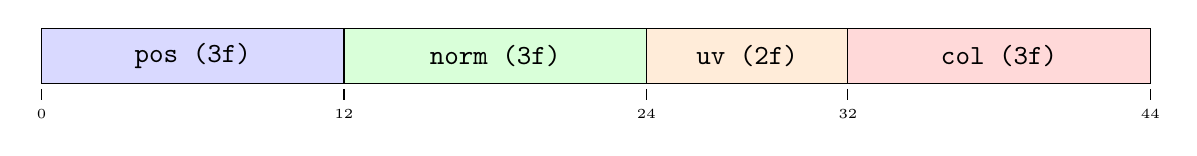
\begin{tikzpicture}[x=0.32cm, y=0.7cm]
  \draw[fill=blue!15]   (0,0)  rectangle (12,1); \node at (6,0.5)  {\texttt{pos (3f)}};
  \draw[fill=green!15]  (12,0) rectangle (24,1); \node at (18,0.5) {\texttt{norm (3f)}};
  \draw[fill=orange!15] (24,0) rectangle (32,1); \node at (28,0.5) {\texttt{uv (2f)}};
  \draw[fill=red!15]    (32,0) rectangle (44,1); \node at (38,0.5) {\texttt{col (3f)}};
  \foreach \x/\lbl in {0/0, 12/12, 24/24, 32/32, 44/44} {
    \draw (\x,-0.1) -- (\x,-0.3);
    \node[below] at (\x,-0.3) {\tiny\lbl};
  }
\end{tikzpicture}
\end{center}

Vertex buffer: $50 \times 44 = 2200$ bytes.
Index buffer: $192 \times 4 = 768$ bytes.
Interleaving keeps all attributes for one vertex in a single cache line.
Conceptually, building a VBO this way resembles allocating a small memory arena:
a single contiguous block is reserved up front, and heterogeneous data
(positions, normals, texture coordinates, colours) is packed into it at
explicit byte offsets---much like manual struct layout in an arena allocator.

% ----------------------------------------------------------------------
\subsection{Native OpenGL Calls}
% ----------------------------------------------------------------------

\begin{lstlisting}[caption={VBO/VAO/EBO setup}]
GLuint vao, vbo, ebo;

glGenVertexArrays(1, &vao);
glBindVertexArray(vao);

glGenBuffers(1, &vbo);
glBindBuffer(GL_ARRAY_BUFFER, vbo);
glBufferData(GL_ARRAY_BUFFER, 2200, vertices, GL_STATIC_DRAW);

glGenBuffers(1, &ebo);
glBindBuffer(GL_ELEMENT_ARRAY_BUFFER, ebo);
glBufferData(GL_ELEMENT_ARRAY_BUFFER, 768, indices, GL_STATIC_DRAW);

GLsizei stride = 44;
// Attribute 0: position (vec3, offset 0)
glEnableVertexAttribArray(0);
glVertexAttribPointer(0, 3, GL_FLOAT, GL_FALSE, stride, (void*)0);
// Attribute 1: normal (vec3, offset 12)
glEnableVertexAttribArray(1);
glVertexAttribPointer(1, 3, GL_FLOAT, GL_FALSE, stride, (void*)12);
// Attribute 2: texcoord (vec2, offset 24)
glEnableVertexAttribArray(2);
glVertexAttribPointer(2, 2, GL_FLOAT, GL_FALSE, stride, (void*)24);
// Attribute 3: colour (vec3, offset 32)
glEnableVertexAttribArray(3);
glVertexAttribPointer(3, 3, GL_FLOAT, GL_FALSE, stride, (void*)32);

glBindVertexArray(0);
\end{lstlisting}

\begin{lstlisting}[caption={Render and cleanup}]
// Draw
glBindVertexArray(vao);
glDrawElements(GL_TRIANGLES, 192, GL_UNSIGNED_INT, (void*)0);

// Cleanup
glDeleteVertexArrays(1, &vao);
glDeleteBuffers(1, &vbo);
glDeleteBuffers(1, &ebo);
\end{lstlisting}


\nocite{*}
\printbibliography

\end{document}
